\documentclass[11pt,twoside,a4paper]{article}
% http://www-h.eng.cam.ac.uk/help/tpl/textprocessing/latex_maths+pix/node6.html symboles de math
% http://fr.wikibooks.org/wiki/Programmation_LaTeX Programmation latex (wikibook)
%=========================== En-Tete =================================
%--- Insertion de paquetages (optionnel) ---
\usepackage[french]{babel}   % pour dire que le texte est en fran{\'e}ais
\usepackage{a4}	             % pour la taille   
\usepackage[T1]{fontenc}     % pour les font postscript
\usepackage{epsfig}          % pour gerer les images
%\usepackage{psfig}
\usepackage{amsmath, amsthm} % tres bon mode mathematique
\usepackage{amsfonts,amssymb}% permet la definition des ensembles
\usepackage{float}           % pour le placement des figure
\usepackage{verbatim}

\usepackage{longtable} % pour les tableaux de plusieurs pages

\usepackage[table]{xcolor} % couleur de fond des cellules de tableaux

\usepackage{lastpage}

\usepackage{multirow}

\usepackage{multicol} % pour {\'e}crire dans certaines zones en colonnes : \begin{multicols}{nb colonnes}...\end{multicols} 

% \usepackage[top=1.5cm, bottom=1.5cm, left=1.5cm, right=1.5cm]{geometry}
% gauche, haut, droite, bas, entete, ente2txt, pied, txt2pied
\usepackage{vmargin}
\setmarginsrb{0.20cm}{0.20cm}{0.20cm}{0.20cm}{15pt}{3pt}{15pt}{3pt}

\usepackage{lscape} % changement orientation page
%\usepackage{frbib} % enlever pour obtenir references en anglais
% --- style de page (pour les en-tete) ---
\pagestyle{empty}

% % % en-tete et pieds de page configurables : fancyhdr.sty

% http://www.trustonme.net/didactels/250.html

% http://ww3.ac-poitiers.fr/math/tex/pratique/entete/entete.htm
% http://www.ctan.org/tex-archive/macros/latex/contrib/fancyhdr/fancyhdr.pdf
% \usepackage{fancyhdr}
% \pagestyle{fancy}
% % \newcommand{\chaptermark}[1]{\markboth{#1}{}}
% % \newcommand{\sectionmark}[1]{\markright{\thesection\ #1}}
% \fancyhf{}
% \fancyhead[LE,RO]{\bfseries\thepage}
% \fancyhead[LO]{\bfseries\rightmark}
% \fancyhead[RE]{\bfseries\leftmark}
% \fancyfoot[LE]{\thepage /\pageref{LastPage} \hfill
	% TITLE
% \hfill 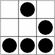
\includegraphics[width=0.5cm]{img/logo_glider.png} }
% \fancyfoot[RO]{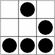
\includegraphics[width=0.5cm]{img/logo_glider.png} \hfill
	% TITLE
% \hfill \thepage /\pageref{LastPage}}
% \renewcommand{\headrulewidth}{0.5pt}
% \renewcommand{\footrulewidth}{0.5pt}
% \addtolength{\headheight}{0.5pt}
% \fancypagestyle{plain}{
	% \fancyhead{}
	% \renewcommand{\headrulewidth}{0pt}
% }


%============================= Corps =================================
\begin{document}

\setlength\parindent{0pt}

\texttt{http://leplus.nouvelobs.com/contribution/1358339-intelligence-artificielle-le-transhumanisme-est-narcissique-visons-l-hyperhumanisme.html}~\\

\textbf{\LARGE Intelligence artificielle : le transhumanisme est narcissique. Visons l'hyperhumanisme} ~\\

\emph{\small Par Jo{\"e}l de Rosnay -- Scientifique, Publi{\'e} le 26-04-2015 {\`a} 12h00 - Modifi{\'e} {\`a} 15h37} ~\\



\begin{minipage}[ht]{7.00cm}
	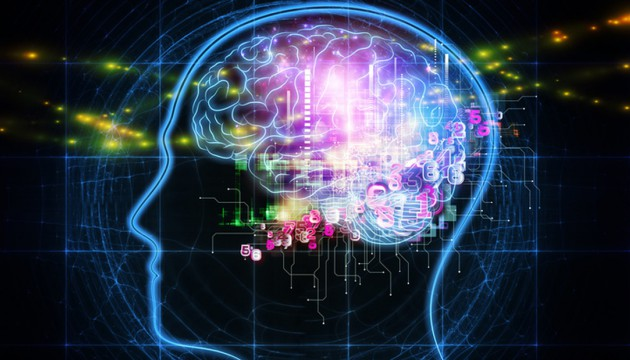
\includegraphics[width=6.95cm]{img/2751429787165.jpg}~\\
	\emph{Le transhumanisme est-il un humanisme ? (Flickr-CC-cblue98)}
\end{minipage} \hfill \begin{minipage}[ht]{0.65\textwidth}
	Temps de lecture Temps de lecture : 7 minutes ~\\

	{\'E}dit{\'e} par \texttt{H{\'e}l{\`e}ne Decommer~\footnotemark}  Auteur parrain{\'e} par \texttt{Dominique Nora~\footnotemark}. ~\\

	\textbf{LE PLUS. L'intelligence des robots et des r{\'e}seaux num{\'e}riques interconnect{\'e}s, {\'e}voluant {\`a} une vitesse exponentielle en relation avec l'{\'e}volution humaine, va ouvrir de nouvelles dimensions du cerveau humain. A condition que les hommes parviennent {\`a} un contr{\^o}le plan{\'e}taire vigilant de l'intelligence artificielle... {\'E}clairage de Jo{\"e}l de Rosnay, scientifique et conseiller de la pr{\'e}sidente d'Universcience (Cit{\'e} des sciences et de l'industrie et Palais de la d{\'e}couverte). } ~\\
\end{minipage}~\\~\\
\footnotetext[1]{\texttt{http://leplus.nouvelobs.com/helenedecommer}}
\footnotetext{\texttt{http://leplus.nouvelobs.com/dnora}}

R{\'e}cemment, des scientifiques et des dirigeants d'entreprises influents d{\'e}claraient publiquement que l'intelligence artificielle (IA) constituait l'une des pires menaces pour l'humanit{\'e}. C'est en tous les cas le \texttt{point de vue de l'astrophysicien Stephen Hawking~\footnotemark}, du fondateur de Microsoft, \texttt{Bill Gates~\footnotemark}, ou encore d'\texttt{Elon Musk~\footnotemark}, cofondateur de Tesla Motors et de SpaceX. ~\\
\footnotetext[3]{\texttt{http://www.20minutes.fr/sciences/1366609-20140504-sous-estimer-intelligence-artificielle-plus-grave-erreur-histoire-stephen-hawking}}
\footnotetext[4]{\texttt{http://lexpansion.lexpress.fr/high-tech/intelligence-artificielle-attention-danger-meme-bill-gates-a-peur\_1647411.html}}
\footnotetext{\texttt{http://www.numerama.com/magazine/31068-elon-musk-voit-l-intelligence-artificielle-comme-une-menace-pour-l-humanite.html}}
	
Atteint de la maladie de Charcot (dystrophie neuromusculaire) Stephen Hawking, qui communique pourtant avec le monde ext{\'e}rieur gr{\^a}ce {\`a} un ordinateur synth{\'e}tiseur de voix, actionn{\'e} par le mouvement de ses yeux, explique que l'IA risque de conduire l'humanit{\'e} {\`a} sa perte parce que les ordinateurs et les robots devenus plus intelligents que l'Homme finiront par le r{\'e}duire {\`a} l'esclavage. M{\^e}me discours alarmiste du c{\^o}t{\'e} du fondateur de Microsoft, qui d{\'e}nonce lui aussi le danger de domination de l'IA sur l'humanit{\'e}. Quant au cr{\'e}ateur de la Tesla {\'e}lectrique ou du nuage de satellites qui donnera au monde entier l'acc{\`e}s Internet, il subventionne l'Institute for the Future of Life (l'Institut pour le futur de la vie) {\`a} coups de millions de dollars pour qu'il trouve le moyen de contr{\^o}ler, voire de stopper, l'IA et les robots intelligents. ~\\

\textbf{De nouvelles dimensions plut{\^o}t qu'une domination}~\\

Une erreur souvent commise, notamment par les personnalit{\'e}s cit{\'e}es pr{\'e}c{\'e}demment, est de comparer la vitesse de l'{\'e}volution exponentielle des ordinateurs, r{\'e}seaux neuronaux et robots, {\`a} celle des mutations des neurones du cerveau, qui, elle, serait lin{\'e}aire. On retrouve la c{\'e}l{\`e}bre divergence temporelle entre progression g{\'e}om{\'e}trique et progression arithm{\'e}tique que Malthus avait d{\'e}j{\`a} signal{\'e}e en comparant la vitesse de l'{\'e}volution d{\'e}mographique conduisant {\`a} la surpopulation et celle de la capacit{\'e} de l'humanit{\'e} {\`a} produire suffisamment de nourriture pour sa survie. ~\\

Pourtant, une {\'e}tude approfondie des tendances technico-soci{\'e}tales sugg{\`e}re que l'intelligence de nos cerveaux, interconnect{\'e}s en symbiose avec les robots, l'IA et les r{\'e}seaux num{\'e}riques, est en train d'{\'e}voluer \emph{simultan{\'e}ment} et {\`a} une vitesse exponentielle. Un processus qui pourrait ouvrir de nouvelles dimensions, encore inconnues du cerveau humain, plut{\^o}t que de conduire {\`a} sa domination. Si nous parvenons, bien entendu, {\`a} assurer la compl{\'e}mentarit{\'e} IA/ cerveaux humains interconnect{\'e}s. ~\\

\textbf{Le mythe de Frankenstein}~\\

La premi{\`e}re de nos grandes peurs rel{\`e}ve du biologique et de l'humain : nous craignons que les cr{\'e}ations humaines ne se retournent contre l'Homme. C'est le mythe de Frankenstein. La deuxi{\`e}me peur est li{\'e}e {\`a} la destruction des emplois. Si les robots remplacent progressivement les m{\'e}tiers les moins qualifi{\'e}s et si la qualit{\'e} du travail fourni par l'intelligence artificielle peut rivaliser avec des m{\'e}decins, juristes, journalistes, enseignants... que restera-t-il aux {\^e}tres humains ? D'o{\`u} cette troisi{\`e}me grande peur : la fin du travail. Cr{\'e}ateur de lien social, fondement m{\^e}me de la vie en soci{\'e}t{\'e} et du sens de la vie pour beaucoup, le travail, tel que nous le connaissons aujourd'hui, est menac{\'e}. ~\\

Cette question philosophique et {\'e}thique du travail se pose depuis l'origine de l'humanit{\'e}. Les robots et, plus largement, la robotique, n'{\'e}chappent pas {\`a} ces questionnements. L'Homme s'est toujours m{\'e}fi{\'e} des robots, sauf dans certaines cultures orientales. Au Japon, par exemple, les robots sont consid{\'e}r{\'e}s comme des assistants essentiels {\`a} l'{\'e}volution de l'humanit{\'e}. Comme pour les robots, "Intelligence artificielle" associe deux mots en apparente contradiction avec l'"intelligence naturelle". Comment l'intelligence, fonction primordiale de nos cerveaux humains pourrait-elle {\^e}tre cr{\'e}{\'e}e de toute pi{\`e}ce ? Une formule "contre nature", qui provoque le rejet. ~\\

Ordinateurs et robots d{\'e}veloppent d{\'e}j{\`a} des capacit{\'e}s d'apprentissage gr{\^a}ce {\`a} toutes les informations disponibles sur les r{\'e}seaux (le Big Data). Les machines intelligentes apprennent ainsi comment fonctionne le monde autour d'elles, comment interagir avec les {\^e}tres vivants (humains et animaux). On peut imaginer que ces robots intelligents soient un jour dot{\'e}s de sensibilit{\'e}, d'empathie, de capacit{\'e} d'abstraction, voire d'intuition... Qualit{\'e}s jusque-l{\`a} r{\'e}serv{\'e}es aux {\^e}tres vivants. --- Doit-on craindre ces cr{\'e}atures "humano{\"i}des" ? Il faut moins craindre l'intelligence artificielle que la stupidit{\'e} naturelle... En d'autres termes, l'{\'e}ducation et la formation des humains sont primordiales, autant qu'il est n{\'e}cessaire "d'{\'e}duquer" les robots en parall{\`e}le. ~\\

\textbf{Des peurs irrationnelles, quasi-religieuses}~\\

{\`A} trop personnaliser l'Intelligence artificielle ou le Big Data, on fabrique une sorte de mythe quasi-religieux. On retrouve l{\`a} les vieilles notions de fin du monde, d'apocalypse et de jugement dernier...La notion de "singularit{\'e}" \texttt{ch{\`e}re {\`a} Ray Kurzweil~\footnotemark} a des relents de sacr{\'e}, de "divinit{\'e}". Il y a une vision panth{\'e}iste dans l'Intelligence artificielle et la singularit{\'e}. Or l'intelligence artificielle est encore peu d{\'e}velopp{\'e}e. La \texttt{loi de Moore~\footnotemark} ne s'applique pas {\`a} l'IA. On est loin des algorithmes qui soient capables de sentir, d'avoir de l'intuition, de prendre des d{\'e}cisions {\'e}clair{\'e}es, d'avoir les outils physiques pour menacer les hommes. ~\\
\footnotetext[6]{\texttt{http://rue89.nouvelobs.com/2013/09/15/singularite-lideologie-silicon-valley-valait-milliards-245677}}
\footnotetext{\texttt{http://www.futura-sciences.com/magazines/high-tech/infos/dico/d/informatique-loi-moore-2447/}}

Les adeptes du transhumanisme pensent avoir trouv{\'e} la parade au d{\'e}passement de l'Homme par l'IA en cr{\'e}ant des surhommes et une supra-intelligence individuelle. En cinq d{\'e}cennies, on a vu ainsi {\'e}merger les th{\'e}ories du transhumanisme, avec une acc{\'e}l{\'e}ration au XXIe si{\`e}cle. Ce mot a {\'e}t{\'e} cr{\'e}{\'e} en 1957 par Julian Huxley, fr{\`e}re d'Aldous, auteur du livre "Le meilleur des mondes". En 1998 a {\'e}t{\'e} cr{\'e}{\'e} le WTA (World Transhumanist Association) conduisant {\`a} une v{\'e}ritable \texttt{d{\'e}claration des "droits transhumanistes"~\footnotemark} publi{\'e}e sur internet. ~\\
\footnotetext{\texttt{http://transhumanism.org/languages/french/declaration.htm}}

\textbf{Le transhumanisme est-il un humanisme ?}~\\

Le transhumanisme consid{\'e}rant l'am{\'e}lioration par la transformation individuelle, conduit-il {\`a} une impasse en se concentrant sur l'individu ? Le transhumain n'ouvre-t-il pas la voix {\`a} l'inhumain ? Et surtout, le transhumanisme est-il un humanisme ? Rappelons qu'on d{\'e}signe par humanisme toute pens{\'e}e qui met au premier plan de ses pr{\'e}occupations le d{\'e}veloppement des qualit{\'e}s essentielles de l'{\^e}tre humain. L'humanisme repose sur la capacit{\'e} {\`a} d{\'e}terminer le bien et le mal en se fondant sur des qualit{\'e}s humaines universelles, en particulier la rationalit{\'e}. C'est l'affirmation de la dignit{\'e} et de la valeur de tous les individus. C'est la raison pour laquelle on peut douter du caract{\`e}re humaniste du transhumanisme qui appara{\^i}t plut{\^o}t comme une d{\'e}marche {\'e}litiste, {\'e}go{\"i}ste et narcissique. ~\\

{\'E}litiste, parce que les transformations pr{\'e}vues sur le corps ou le cerveau sont r{\'e}serv{\'e}es {\`a} quelques privil{\'e}gi{\'e}s disposant de moyens financiers, leur permettant d'int{\'e}grer de nouvelles capacit{\'e}s ou de subir des modifications. --- {\'E}go{\"i}ste, parce que tout ce qui vient de la nature doit retourner {\`a} la nature. Dans tous les aspects de l'{\'e}volution, on constate que la vie et la mort sont indissociables et indispensables l'une {\`a} l'autre. --- Narcissique parce que la qu{\^e}te d'immortalit{\'e} risque de conduire {\`a} un monde de conflit entre les jeunes g{\'e}n{\'e}rations et les anciennes en comp{\'e}tition pour l'acc{\`e}s aux ressources et au pouvoir. On verrait surgir la supr{\'e}matie des surhommes sur les sous-hommes, des Alphas sur les Gammas...Si la tentation de la domination d'une caste sur une autre et de l'eug{\'e}nisme ne sont jamais loin, on se doit de respecter les avanc{\'e}es transhumanistes car elles peuvent mener, gr{\^a}ce {\`a} une r{\'e}flexion philosophique critique et constructive, {\`a} repousser les limites du corps humain, {\`a} allonger l'esp{\'e}rance de vie et contribuer {\`a} une {\'e}volution humaine et soci{\'e}tale positive. B{\'e}n{\'e}ficiant, gr{\^a}ce aux NBIC ((nanotechnologie, biotechnologie, infotechnologie et science cognitive)) d'une symbiose entre biologie-m{\'e}canique-{\'e}lectronique et num{\'e}rique. ~\\

En effet, avec les progr{\`e}s de la biologie et du num{\'e}rique, la fronti{\`e}re entre humains, m{\'e}canique et {\'e}lectronique dispara{\^i}t progressivement. Gr{\^a}ce {\`a} la neurobiologie synth{\'e}tique, l'Homme peut entrer en symbiose de plus en plus {\'e}troite avec les machines num{\'e}riques et tirer un b{\'e}n{\'e}fice de sa compl{\'e}mentarit{\'e} avec les robots et l'intelligence artificielle. D{\'e}j{\`a}, les objets connect{\'e}s dans l'{\'e}cosyst{\`e}me num{\'e}rique (IOT ou l'Internet des objets) agissent en {\'e}troite symbiose avec les humains. Ils cr{\'e}ent ainsi un macro-organisme plan{\'e}taire qui a ses fonctionnalit{\'e}s propres dans sa capacit{\'e} {\`a} traiter les informations. ~\\

J'ai d{\'e}crit cette hybridation de plus en plus {\'e}troite, entre les {\^e}tres humains et les machines num{\'e}riques, dans "L'Homme symbiotique" (Seuil, 1995). J'appelais ce macro-organisme plan{\'e}taire, le "Cybionte", produit du mariage de la cybern{\'e}tique et de la biologie. Une hypoth{\`e}se aujourd'hui partag{\'e}e par des scientifiques et philosophes de la complexit{\'e}, notamment dans le cadre du Global Brain Institute (GBI). Il n'y {\'e}tait pas question de l'av{\`e}nement de cyborg, d'homme bionique ou de Superman, mais bien d'un humain, "symbiotique", reli{\'e} {\`a} un macro-organisme plan{\'e}taire construit de l'int{\'e}rieur, dont nous constituerions les cellules et les neurones. ~\\
\footnotetext{\texttt{http://www.globalbraininstitute.org/}}

\textbf{Une autre voie est possible, l'hyperhumanisme}~\\

C'est {\`a} ce stade que l'intelligence artificielle peut aider {\`a} ouvrir une autre voie. Une voie qui permettrait de d{\'e}passer le caract{\`e}re individualiste, {\'e}litiste ou {\'e}go{\"i}ste des promoteurs du transhumanisme, c'est-{\`a}-dire de consid{\'e}rer \emph{l'int{\'e}gration des humains et leur symbiose} plut{\^o}t que leur transformation individuelle. ~\\

Imaginons que l'esp{\`e}ce humaine parvienne {\`a} faire un saut quantitatif et qualitatif, au-del{\`a} du \emph{transhumanisme}, vers ce que j'appellerai l'\emph{hyperhumanisme}. Au-del{\`a} d'une <<philosophie>> qui se concentre exclusivement sur l'individu et semble d{\'e}nier {\`a} la collectivit{\'e} les capacit{\'e}s d'{\'e}voluer en compl{\'e}mentarit{\'e} et en symbiose avec les machines num{\'e}riques et l'intelligence artificielle, c'est, au contraire, vers la symbiose \emph{int{\'e}gr{\'e}e} et \emph{collective} que doit se diriger l'humanit{\'e}. Et c'est l{\`a} tout le d{\'e}fi que devront relever les Terriens du III{\`e}me mill{\'e}naire. ~\\

Le Cybionte a commenc{\'e} {\`a} vivre en symbiose avec nous : nous lui sous-traitons d{\'e}j{\`a} des probl{\`e}mes d'une tr{\`e}s grande complexit{\'e} (m{\'e}t{\'e}orologie, op{\'e}rations boursi{\`e}res, trafic routier...) que nos cerveaux et nos ordinateurs individuels sont incapables de traiter en temps r{\'e}el. Cette symbiose Homme/Cybionte va se d{\'e}velopper {\`a} une vitesse exponentielle faisant de nous, par une sorte de transmutation, des mutants d'un nouvel {\^a}ge, ou plut{\^o}t des \emph{transmutants}. Il ne s'agit pas de devenir des \emph{transhumains}, mais des \emph{suprahumains} pour entrer dans l'{\^a}ge de l'hyper-humanisme plut{\^o}t que dans celui du transhumanisme. Les caract{\`e}res humains pourraient {\^e}tre encore plus d{\'e}velopp{\'e}s et encore plus \emph{humains} que ne l'a produit l'{\'e}volution. ~\\

De telles lois existent dans la nature. On les appelle les lois d'int{\'e}gration diff{\'e}rentiation. Dans le corps humain, un globule rouge, un globule blanc ou une cellule de foie sont beaucoup plus "elles-m{\^e}mes" que dans une bo{\^i}te de p{\'e}tri surnageant dans un milieu nutritif pos{\'e}e sur la paillasse d'un laboratoire. Notre corps est constitu{\'e} de 6000 milliards de cellules, mille fois plus que d'{\^e}tres humains sur la plan{\`e}te. L'ensemble de nos cellules et des microbes utiles que nous h{\'e}bergeons en symbiose (le microbiome), constitue un m{\'e}ta-g{\'e}nome que les chercheurs sont en train de d{\'e}crypter. Chaque cellule du corps, chaque microbe du microbiome repr{\'e}sente toutes les fonctionnalit{\'e}s que leur permet leur g{\'e}nome et son expression au sein d'une soci{\'e}t{\'e} ou d'un {\'e}cosyst{\`e}me int{\'e}gr{\'e}, beaucoup plus efficacement que s'ils {\'e}taient isol{\'e}s. ~\\

Ce parall{\`e}le montre qu'une symbiose conduisant {\`a} l'hyper humanisme pourrait d{\'e}velopper \emph{d'autres dimensions du cerveau} aujourd'hui occult{\'e}es ou inhib{\'e}es par la concurrence, la comp{\'e}tition, la n{\'e}cessit{\'e} de survie dans un monde parfois hostile et organis{\'e} pour la survie de l'individu plut{\^o}t que la coop{\'e}ration, la solidarit{\'e}, l'altruisme et le partage. ~\\

\textbf{Une sorte d'immortalit{\'e} virtuelle}~\\

Alors que beaucoup craignaient la banalisation de l'Homme, int{\'e}gr{\'e} {\`a} un plus grand que lui dans le cadre d'une {\'e}troite symbiose, ce serait au contraire l'hyperhumanit{\'e} et l'hyper-humanisme qui prendraient le pas sur l'Homme asservi ou domin{\'e}. Il est possible que des sentiments comme la fraternit{\'e}, l'altruisme, la volont{\'e} d'aide, d'empathie, de respect et de solidarit{\'e}... se d{\'e}veloppent d'une mani{\`e}re que nous n'imaginons pas encore. ~\\

Le capital d'id{\'e}es et de connaissances accumul{\'e} au fil des mill{\'e}naires par l'humanit{\'e} pourrait {\^e}tre l{\'e}gu{\'e} aux nouvelles g{\'e}n{\'e}rations et offrir {\`a} chacun une sorte d'immortalit{\'e} virtuelle. Ainsi, il ne s'agit plus de viser l'immortalit{\'e} biologique, comme en r{\^e}vent les transhumanistes, mais d'atteindre l'immortalit{\'e} virtuelle en faisant en sorte que l'humanit{\'e} dans son ensemble, l'hyperhumanit{\'e}, b{\'e}n{\'e}ficie pratiquement en temps r{\'e}el de toutes les innovations et cr{\'e}ations, fruit des activit{\'e}s et r{\'e}flexions des {\^e}tres humains connect{\'e}s {\`a} cette intelligence collective, point ultime du d{\'e}veloppement de la complexit{\'e} et de la conscience vers lequel se dirige l'univers. Un point Om{\'e}ga, plut{\^o}t qu'un point de Singularit{\'e}. ~\\

\emph{Tribune tir{\'e}e d'une conf{\'e}rences faite sur "L'utopie de transhumanisme" au GODF (Grand Orient de France) le 3 f{\'e}vrier 2015. }

\end{document}
